\documentclass{article}

\usepackage{amsmath, amsfonts, amssymb, amstext, amscd, amsthm, bbm, CJKutf8, color, dsfont, enumerate, float, graphicx, hyperref, makeidx, mathrsfs, mathtools, marvosym, soul, url, verbatim, xcolor, xfrac}
\usepackage[left=2cm,top=2cm,right=2cm,bottom=2cm,bindingoffset=0cm]{geometry}
\hypersetup{
    colorlinks=true,
    linkcolor=black!50!red,
    urlcolor=black!50!red
}
\allowdisplaybreaks

\newenvironment{subproof}[1][Proof]
    {\proof[#1]\leftskip=1cm\rightskip=1cm}
	{\endproof}

%theorems with custom numbering
%\newtheorem{innerthm}{Theorem}
%\newenvironment{thm}[1]
    %{\renewcommand\theinnerthm{#1}\innercustomthm}
    %{\endinnerthm}

\newtheorem{theorem}{Theorem}
\newtheorem{lemma}{Lemma}
\newtheorem{proposition}{Proposition}
\newtheorem{corollary}{Corollary}
\newtheorem{claim}{Claim}
\newtheorem{conjecture}{Conjecture}
\newtheorem{justification}{Justification}
\newtheorem{definition}{Definition}
\newtheorem*{remark}{Remark}
\newtheorem*{note}{Note}

\renewcommand{\restriction}[1]{\downharpoonright_{#1}}
\renewcommand{\qedsymbol}{QED}
\renewcommand{\leq}{\leqslant}
\renewcommand{\geq}{\geqslant}
\renewcommand{\and}{~\wedge~}
\newcommand{\defn}{\coloneqq}
\newcommand{\disj}{~\vee~}
\newcommand{\xor}{~\oplus~}
\newcommand{\divides}{~|~}
\newcommand{\given}{\middle|}
\newcommand{\suchthat}{~\middle|~}
\newcommand{\contradiction}{~\text{\Large \Lightning}}
\newcommand{\conj}[1]{\overline{#1}}
\newcommand{\mean}[1]{\overline{#1}}
\newcommand{\integral}[1]{\smashoperator{\int_{#1}}}
\newcommand*\diff{\mathop{}\!\mathrm{d}}
\newcommand{\E}[1]{\mathbb{E}\sqparens*{#1}}
\newcommand{\Esub}[2]{\mathbb{E}_{#1}\sqparens*{#2}}
\newcommand{\var}[1]{\mathrm{Var}\parens*{#1}}
\newcommand{\cov}[2]{\mathrm{Cov}\parens*{#1, #2}}
\newcommand{\der}[2]{\frac{\diff{#1}}{\diff{#2}}}
\newcommand{\dern}[3]{\frac{\diff^{#3}{#1}}{\diff{#2}^{#3}}}
\newcommand{\derm}[3]{\frac{\diff^{#3}{#1}}{\diff{#2}}}
\newcommand{\prt}[2]{\frac{\partial{#1}}{\partial{#2}}}
\newcommand{\prtn}[3]{\frac{\partial^{#3}{#1}}{\partial{#2}^{#3}}}
\newcommand{\prtm}[3]{\frac{\partial^{#3}{#1}}{\partial{#2}}}

\DeclareMathOperator{\lcm}{lcm}
\DeclareMathOperator*{\argmin}{arg\!\min}
\DeclareMathOperator*{\argmax}{arg\!\max}

\let\originalleft\left
\let\originalright\right
\renewcommand{\left}{\mathopen{}\mathclose\bgroup\originalleft}
\renewcommand{\right}{\aftergroup\egroup\originalright}
\newcommand{\zh}[1]{\begin{CJK}{UTF8}{gbsn}#1\end{CJK}}
\newcommand{\jp}[1]{\begin{CJK}{UTF8}{gbsn}#1\end{CJK}}

\DeclarePairedDelimiterX \inner[2]{\langle}{\rangle}{#1,#2}
\DeclarePairedDelimiterX \braket[2]{\langle}{\rangle}{#1 \delimsize\vert #2}
\DeclarePairedDelimiter \bra{\langle}{\rvert}
\DeclarePairedDelimiter \ket{\lvert}{\rangle}
\DeclarePairedDelimiter \abs{\lvert}{\rvert}
\DeclarePairedDelimiter \norm{\lVert}{\rVert}
\DeclarePairedDelimiter \set{\lbrace}{\rbrace}
\DeclarePairedDelimiter \seq{\langle}{\rangle}
\DeclarePairedDelimiter \parens{(}{)}
\DeclarePairedDelimiter \sqparens{[}{]}

\begin{document}
\begin{center}
	\textsc{\huge Monte Carlo Methods}\\
	\textsc{\Large Homework 1}\\
\end{center}
\begin{flushright}
	Daniel Gonzalez\\
    $30$\textsuperscript{th} of January, $2019$
\end{flushright}

\section{Problems}
\begin{enumerate}
    \item
        {\it Given a Linear Congruential Generator with parameters $a, c, m \in \mathbb{Z}$, show using mathematical induction that
        \begin{equation*}
            x_{n+k} \equiv a^k x_n + \frac{a^k - 1}{a-1}c \mod{m}
        \end{equation*}
        where $a \geq 2$ and $k \geq 0$.
        This shows that the $(n+k)$\textsuperscript{th} sequence term can be directly computed from the $n$\textsuperscript{th}.}
        \begin{proof}
            A Linear Congruential Generator is a sequence $\seq{x_n}$ with parameters $a, c, m \in \mathbb{Z}$ defined by
            \begin{equation*}
                x_{n+1} \equiv ax_n + c \mod{m}.
            \end{equation*}
            We will prove the claim by induction on $k \in \mathbb{N}$.
            Let $a \geq 2$ and $n \in \mathbb{N}$ and observe that, when $k = 0$, we trivially have
            \begin{equation*}
                x_{n + 0} = 1x_n + \frac{1 - 1}{a - 1}c \equiv a^0x_n + \frac{a^0 - 1}{a - 1}c \mod{m}.
            \end{equation*}
            Now, assume that the claim is true for some $k \in \mathbb{N}$.
            Observe that
            \begin{alignat*}{2}
                x_{n + (k+1)} &\equiv ax_{n + k} + c &&\mod{m}\\
                &\equiv a\parens*{a^kx_{n} + \frac{a^k - 1}{a - 1}c} + c &&\mod{m}\\
                &\equiv a^{k+1}x_n + \frac{a^{k+1} - a}{a - 1}c + \frac{a - 1}{a - 1}c &&\mod{m}\\
                &\equiv a^{k+1}x_n + \frac{a^{k+1} - 1}{a - 1}c &&\mod{m}.
            \end{alignat*}
            Therefore, for all $n \in \mathbb{N}$ and $k \in \mathbb{N}$, we can conclude that $a \geq 2$ implies
            \begin{equation*}
                x_{n+k} \equiv a^kx_n + \frac{a^k - 1}{a - 1}c \mod{m}.
            \end{equation*}
        \end{proof}
    \item
        {\it Write a code that implements RANDU. For debugging purposes, print $x_{1000}$ when the seed is $x_0 = 1$.}
        \begin{enumerate}
            \item
                {\it Using RANDU generate $u_1, u_2, \dots u_{20002}$ where $u_n \defn \sfrac{x_n}{2^{31}}$.
                For all triples $\parens*{u_i, u_{i+1}, u_{i+2}}$ such that $0.5 \leq u_{i+1} \leq 0.51$, plot the points $\parens*{u_i, u_{i+1}}$.
                Comment on the pattern of your scatter plot.}

                The RANDU pseudorandom number generator was implemented in \texttt{randu.hs} using \href{https://www.haskell.org/}{Haskell}.
                The \texttt{randu} function takes an integer input and outputs the next element of the RANDU sequence,
                modified so that if $x_1 = 1$ is input, then $x_{1000} = 649091873$ is output.
                The \texttt{randuSeq} function takes an initial seed and a length parameter and generates the RANDU sequence of that length determined by that seed.
                The \texttt{uSeq} function then takes a list, such as the RANDU sequence, and divides every element of the list by $2^{31}$, the modulus used for RANDU.

                The \texttt{partA} function constructs a list $[u_1, u_2, \dots u_{20002}]$ using \texttt{uSeq},
                on which the \texttt{parse} function acts to produce a list of ordered pairs $\parens*{u_i, u_{i+1}}$ such that $0.5 \leq u_{i+1} \leq 0.51$.
                These lists of ordered pairs were computed for seeds $x_1 \in \set*{3, 5, 7, 9, 101}$ and then plotted by \texttt{graph.py} using
                \href{https://matplotlib.org/}{matplotlib} with Python
                (and \href{https://seaborn.pydata.org/index.html}{seaborn} for aesthetics).
                The following figure shows the resulting plot.
                As we can clearly see, the points all lie on $10$ parallel planes in $\mathbb{R}^2$.
                This shows that, even across different seeds, the RANDU sequence is highly nonrandom.
                When a value $x_i$ in a RANDU sequence is observed to satisfy $0.5 \leq x_i \leq 0.51$,
                we can immediately deduce that the values $x_{i-1}$ and $x_{i+1}$ lie on one of these $10$ planes.
                \begin{figure}[H]
                    \begin{minipage}{\textwidth}
                        \centering
                        \caption{Modified RANDU}
                        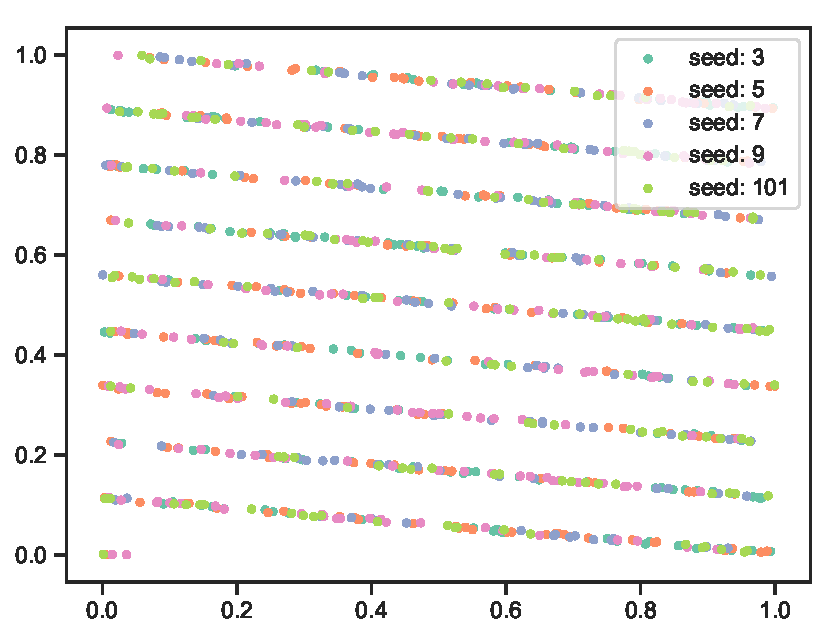
\includegraphics[scale=0.8]{../figures/randu.pdf}
                    \end{minipage}
                \end{figure}
            \item
                {\it Generate a sequence of length $1002$.
                Use a program that plots points in $3$ dimensions and rotates the axes to rotate the points until you can see the $15$ planes.}

                Using the \texttt{partB} function in the same $\texttt{randu.hs}$ Haskell file,
                the standard RANDU sequence $x_1, x_2, \dots x_{1002}$ was computed with $x_1 = 3$.
                The \texttt{triples} function then generated $\parens*{x_1, x_2, x_3}, \parens*{x_2, x_3, x_4}, \dots \parens*{x_{1000}, x_{1001}, x_{1002}}$,
                which was plotted using the \href{https://cran.r-project.org/web/packages/plot3D/index.html}{plot3D} library for R.
                The following are $15$ plots highlighting the $15$ different planes that the RANDU points lie on in $\mathbb{R}^3$.
                \begin{figure}[H]
                    \centering
                    \begin{minipage}{.3\textwidth}
                        \centering
                        \caption{RANDU plane 1}
                        \includegraphics[scale=0.3]{../figures/RANDU_plane1.pdf}
                    \end{minipage}
                    \begin{minipage}{.3\textwidth}
                        \centering
                        \caption{RANDU plane 2}
                        \includegraphics[scale=0.3]{../figures/RANDU_plane2.pdf}
                    \end{minipage}
                    \begin{minipage}{.3\textwidth}
                        \centering
                        \caption{RANDU plane 3}
                        \includegraphics[scale=0.3]{../figures/RANDU_plane3.pdf}
                    \end{minipage}
                \end{figure}
                \begin{figure}[H]
                    \centering
                    \begin{minipage}{.3\textwidth}
                        \centering
                        \caption{RANDU plane 4}
                        \includegraphics[scale=0.3]{../figures/RANDU_plane4.pdf}
                    \end{minipage}
                    \begin{minipage}{.3\textwidth}
                        \centering
                        \caption{RANDU plane 5}
                        \includegraphics[scale=0.3]{../figures/RANDU_plane5.pdf}
                    \end{minipage}
                    \begin{minipage}{.3\textwidth}
                        \centering
                        \caption{RANDU plane 6}
                        \includegraphics[scale=0.3]{../figures/RANDU_plane6.pdf}
                    \end{minipage}
                \end{figure}
                \begin{figure}[H]
                    \centering
                    \begin{minipage}{.3\textwidth}
                        \centering
                        \caption{RANDU plane 7}
                        \includegraphics[scale=0.3]{../figures/RANDU_plane7.pdf}
                    \end{minipage}
                    \begin{minipage}{.3\textwidth}
                        \centering
                        \caption{RANDU plane 8}
                        \includegraphics[scale=0.3]{../figures/RANDU_plane8.pdf}
                    \end{minipage}
                    \begin{minipage}{.3\textwidth}
                        \centering
                        \caption{RANDU plane 9}
                        \includegraphics[scale=0.3]{../figures/RANDU_plane9.pdf}
                    \end{minipage}
                \end{figure}
                \begin{figure}[H]
                    \centering
                    \begin{minipage}{.3\textwidth}
                        \centering
                        \caption{RANDU plane 10}
                        \includegraphics[scale=0.3]{../figures/RANDU_plane10.pdf}
                    \end{minipage}
                    \begin{minipage}{.3\textwidth}
                        \centering
                        \caption{RANDU plane 11}
                        \includegraphics[scale=0.3]{../figures/RANDU_plane11.pdf}
                    \end{minipage}
                    \begin{minipage}{.3\textwidth}
                        \centering
                        \caption{RANDU plane 12}
                        \includegraphics[scale=0.3]{../figures/RANDU_plane12.pdf}
                    \end{minipage}
                \end{figure}
                \begin{figure}[H]
                    \centering
                    \begin{minipage}{.3\textwidth}
                        \centering
                        \caption{RANDU plane 13}
                        \includegraphics[scale=0.3]{../figures/RANDU_plane13.pdf}
                    \end{minipage}
                    \begin{minipage}{.3\textwidth}
                        \centering
                        \caption{RANDU plane 14}
                        \includegraphics[scale=0.3]{../figures/RANDU_plane14.pdf}
                    \end{minipage}
                    \begin{minipage}{.3\textwidth}
                        \centering
                        \caption{RANDU plane 15}
                        \includegraphics[scale=0.3]{../figures/RANDU_plane15.pdf}
                    \end{minipage}
                \end{figure}
        \end{enumerate}
    \item
        {\it Download a code for the Mersenne Twister written by Mutsuo Saito and Makoto Matsumoto.
        Generate $1002$ numbers, and plot pairs and triples of successive numbers for a visual inspection of randomness. Discuss your conclusions.}

        Though there are many implementations of the Mersenne Twister available for Haskell,
        the SIMD Fast Mersenne Twister found in \href{https://hackage.haskell.org/package/mersenne-random}{System.Random.Mersenne}
        was chosen for its efficiency and the clarity of its documentation.

        The \texttt{mersenne.hs} file implements the \texttt{mersenne} function,
        which generates numbers in $[0, 1)$ using the aforementioned Mersenne Twister seeded by the current system time.
        The \texttt{mersenneList} function then (lazily) constructs an infinite sequence of numbers using \texttt{mersenne}, from which the first $n$ are taken.
        These $n$ numbers are then arranged into a list of either pairs or triples by the \texttt{pairs} and \texttt{triples} functions.

        The following two figures are plots of the same sequence of $1002$ numbers,
        generated in the manner described above, split into a sequences of pairs and triples respectively.
        As we can clearly see, the plots appear completely random and there is no readily apparent structure in the data from visual inspection.
        \begin{figure}[H]
            \begin{minipage}{\textwidth}
                \centering
                \caption{Mersenne Twister in 2D}
                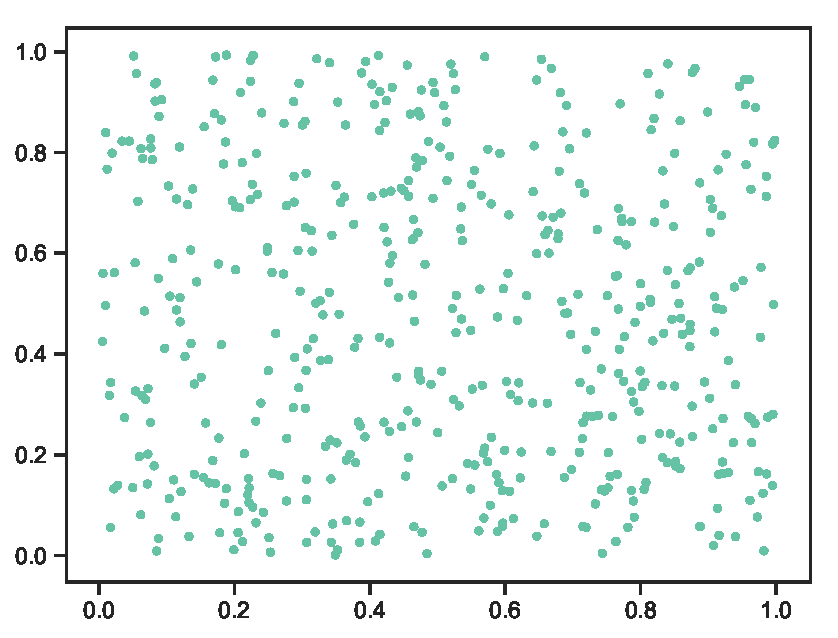
\includegraphics[scale=0.9]{../figures/mersenne2D.pdf}
            \end{minipage}
        \end{figure}
        \begin{figure}[H]
            \begin{minipage}{\textwidth}
                \centering
                \caption{Mersenne Twister in 3D}
                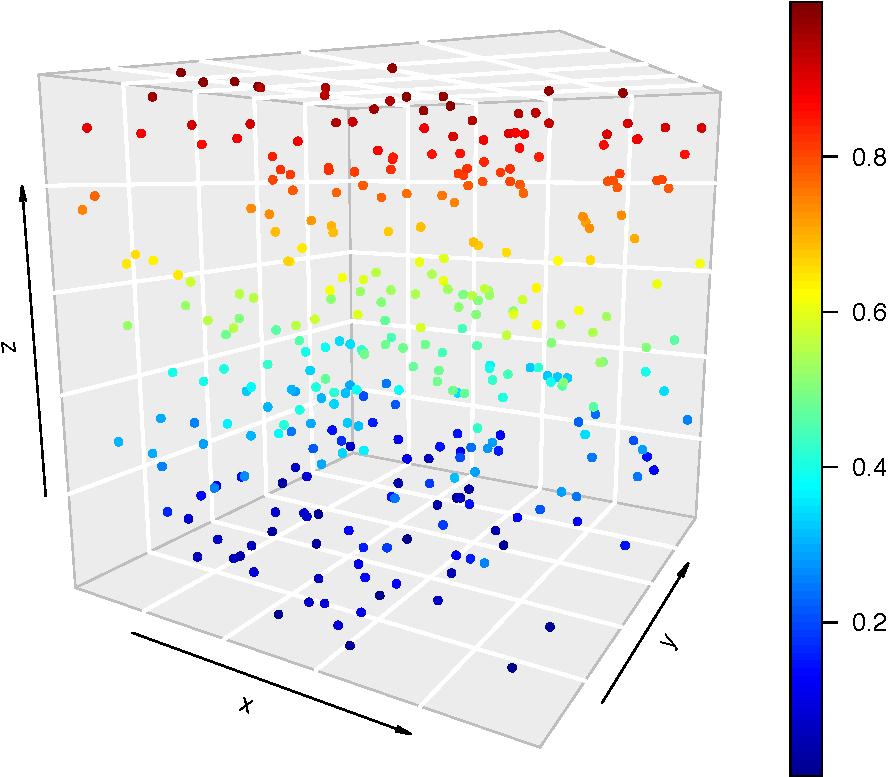
\includegraphics[scale=0.9]{../figures/mersenne3D.pdf}
            \end{minipage}
        \end{figure}
    \item
        {\it Write a computer code for the Halton sequence.
        The input should be the dimension $s$ and $n$, and the output should be the $n$\textsuperscript{th} Halton vector where the bases are the first $s$ primes.
        Then, generate $1000$ two-dimensional Halton vectors and plot them.
        Also plot $1000$ two-dimensional vectors obtained by the Mersenne Twister.
        Can you make any observations comparing the two plots visually?}

        The \texttt{halton.hs} file implements multi-dimensional Halton sequences where the basis along dimension $i$ is the $i$\textsuperscript{th} prime number.
        First, the \texttt{primes} function generates an infinite list of all prime numbers (lazily evaluated, thanks to Haskell).
        The \texttt{haltonList} function takes two parameters, the dimension $s$ and the length of the list $n$,
        and then takes $s$ primes from the list generated by \texttt{primes} and computes $n$ terms of the Halton sequence for each prime.
        The resulting sequences are arranged into lists of length $s$ and returned to the user as a sequence of $n$ such lists.

        Using the parameters $s = 2$ and $n = 1000$, a list of $1000$ two-dimensional Halton vectors was computed in the above fashion.
        This two-dimensional data is plotted below against $1000$ points generated by the Mersenne Twister from the previous problem.
        We can observe that the Halton sequence seems to fill the space $[0, 1] \times [0, 1]$ more evenly than the Mersenne sequence,
        which appears to occasionally clump together into small clusters of between 3 and 6 points.
        \begin{figure}[H]
            \begin{minipage}{\textwidth}
                \centering
                \caption{2D Halton Sequence}
                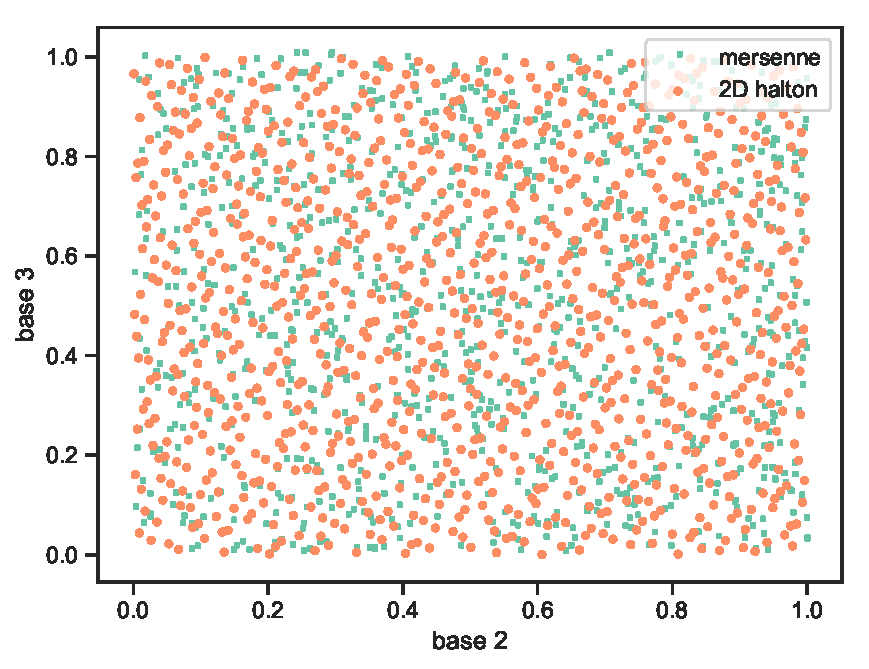
\includegraphics[scale=0.9]{../figures/halton.pdf}
            \end{minipage}
        \end{figure}
    \item
        {\it Consider the quadrature problem $\int_{0}^{1}e^x\diff{x}$.
        You will estimate this integral using Monte Carlo and Random Quasi-Monte Carlo methods by computing $\theta_k \defn \frac{1}{N}\sum_{i = 1}^{N}e^{x_i}$,
        where the subscript $k$ refers to the $k$\textsuprscript{th} estimate.}
        \begin{enumerate}
            \item
                {\it Use Mersenne Twister to obtain $\theta_1, \theta_2, \dots \theta_m$ where $m = 40$ and $N = 1000$.
                Compute the mean and standard deviation of the estimates.}
            \item
                {\it Use random shifted Halton sequences to obtain $\theta_1, \theta_2, \dots \theta_m$ where $m = 40$ and $N = 1000$.
                Compute the mean and standard deviation of the estimates.}
            \item
                {\it Repeat parts} (a) {\it and} (b) {\it with $N = 10000$.}
            \item
                {\it Compute the exact value of the integral.
                Present all of the above data together to create a convincing argument for which method is better for approximating the integral.}
        \end{enumerate}

        \newpage
        \begin{table}[]
            \centering
            \begin{tabular}{rcccc}
                \multicolumn{1}{l}{}                             & \multicolumn{2}{c}{MC}                        & \multicolumn{2}{c}{RQMC}           \\ \cline{2-5}
                \multicolumn{1}{r|}{$N$}                         & \multicolumn{1}{c|}{1,000} & \multicolumn{1}{c|}{10,000} & \multicolumn{1}{c|}{1,000} & \multicolumn{1}{c|}{10,000} \\ \cline{2-5} \cline{2-5}
                    \multicolumn{1}{r|}{Abs. Error}                       & \multicolumn{1}{c|}{$6.485 \times 10^{-4}$}      & \multicolumn{1}{c|}{$5.624 \times 10^{-4}$}       & \multicolumn{1}{c|}{$5.907 \times 10^{-5}$}      & \multicolumn{1}{c|}{$1.235 \times 10^{-5}$}       \\ \cline{2-5}
                \multicolumn{1}{r|}{Mean $\mu$}                  & \multicolumn{1}{c|}{1.718930378181906}      & \multicolumn{1}{c|}{1.718844274942174}       & \multicolumn{1}{c|}{1.71822275488340}      & \multicolumn{1}{c|}{1.718294181840698}       \\ \cline{2-5}
                \multicolumn{1}{r|}{Std. Dev. $\sigma$} & \multicolumn{1}{c|}{$1.752 \times 10^{-2}$}      & \multicolumn{1}{c|}{$4.345 \times 10^{-3}$}       & \multicolumn{1}{c|}{$8.024 \times 10^{-4}$}      & \multicolumn{1}{c|}{$9.477 \times 10^{-5}$}       \\ \cline{2-5}
            \end{tabular}
        \end{table}

        The above table summarizes the results of the quadrature methods implemented in the \texttt{MC.hs} and \texttt{RQMC.hs} files.
        The random shifted Halton sequence used for the RQMC estimation is a
        Van der Corput sequence shifted by a number generated by the Mersenne Twister and truncated to lie within $[0, 1]$.
        The value of the integral is $\int_{0}^{1}e^x\diff{x} = e - 1 \approx 1.718281828459045235$, which was used to compute the errors in the table.

        As we can see from the table, the RQMC method produces, with the same number of sample points,
        estimates of the integral which are more accurate by an order of magnitude ($10^{-4}$ versus $10^{-5}$ for MC and RQMC respectively).
        Not only that, but when $N = 1,000$ the RQMC method has a standard deviation an order of magnitude lower than the MC method.
        The same is true for $N = 10,000$, showing that RQMC dominates MC in all metrics when it comes to estimating the integral.
        However, there is a caveat with using RQMC: when estimating with $N = 10,000$, generating the RQMC estimates took more than twice as long as the MC.
        This shows us that the performance of RQMC comes at the cost of computation time.

        These findings are further supported by the following plots, which also summarize the data.
        \begin{figure}[H]
            \begin{minipage}{0.5\textwidth}
                \centering
                \caption{MC vs. RQMC with $N = 1,000$}
                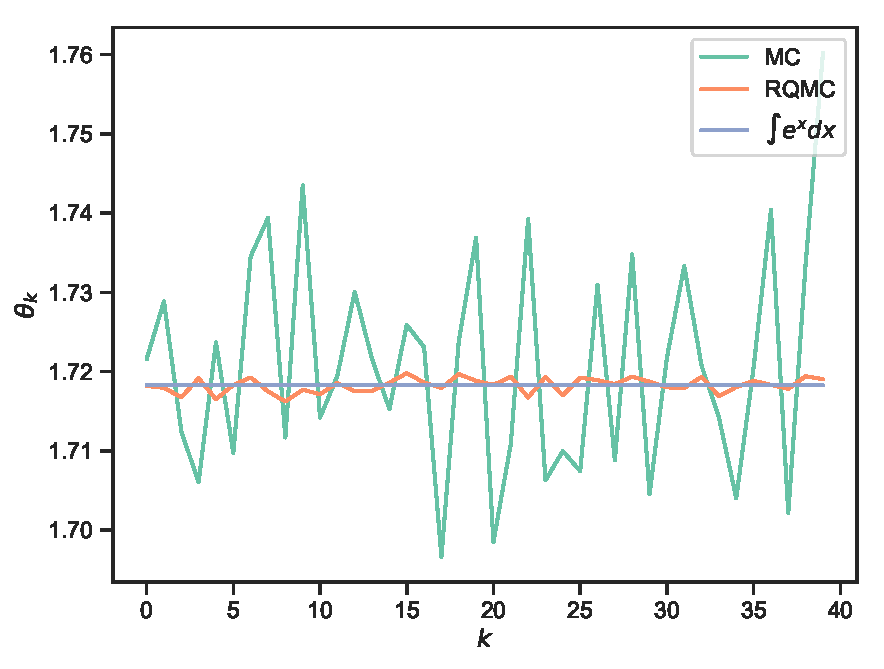
\includegraphics[scale=0.6]{../figures/MC1.pdf}
            \end{minipage}
            \begin{minipage}{0.5\textwidth}
                \centering
                \caption{MC vs. RQMC with $N = 10,000$}
                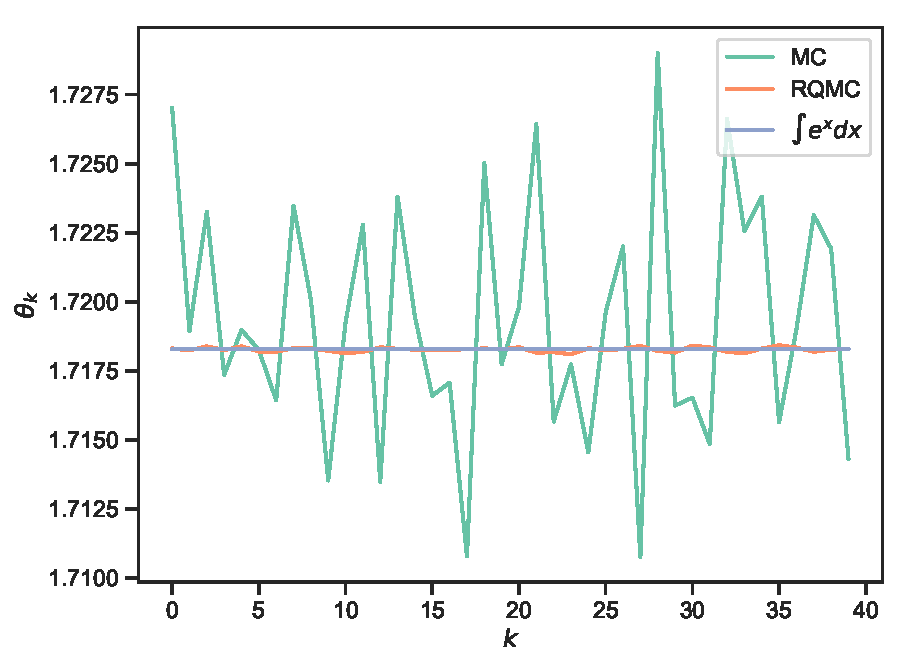
\includegraphics[scale=0.6]{../figures/MC2.pdf}
            \end{minipage}
        \end{figure}

\end{enumerate}

\section{Appendix}
\subsection{RANDU Haskell Code (\texttt{randu.hs})}
    \begin{figure}[H]
        \begin{minipage}{\textwidth}
            \centering
            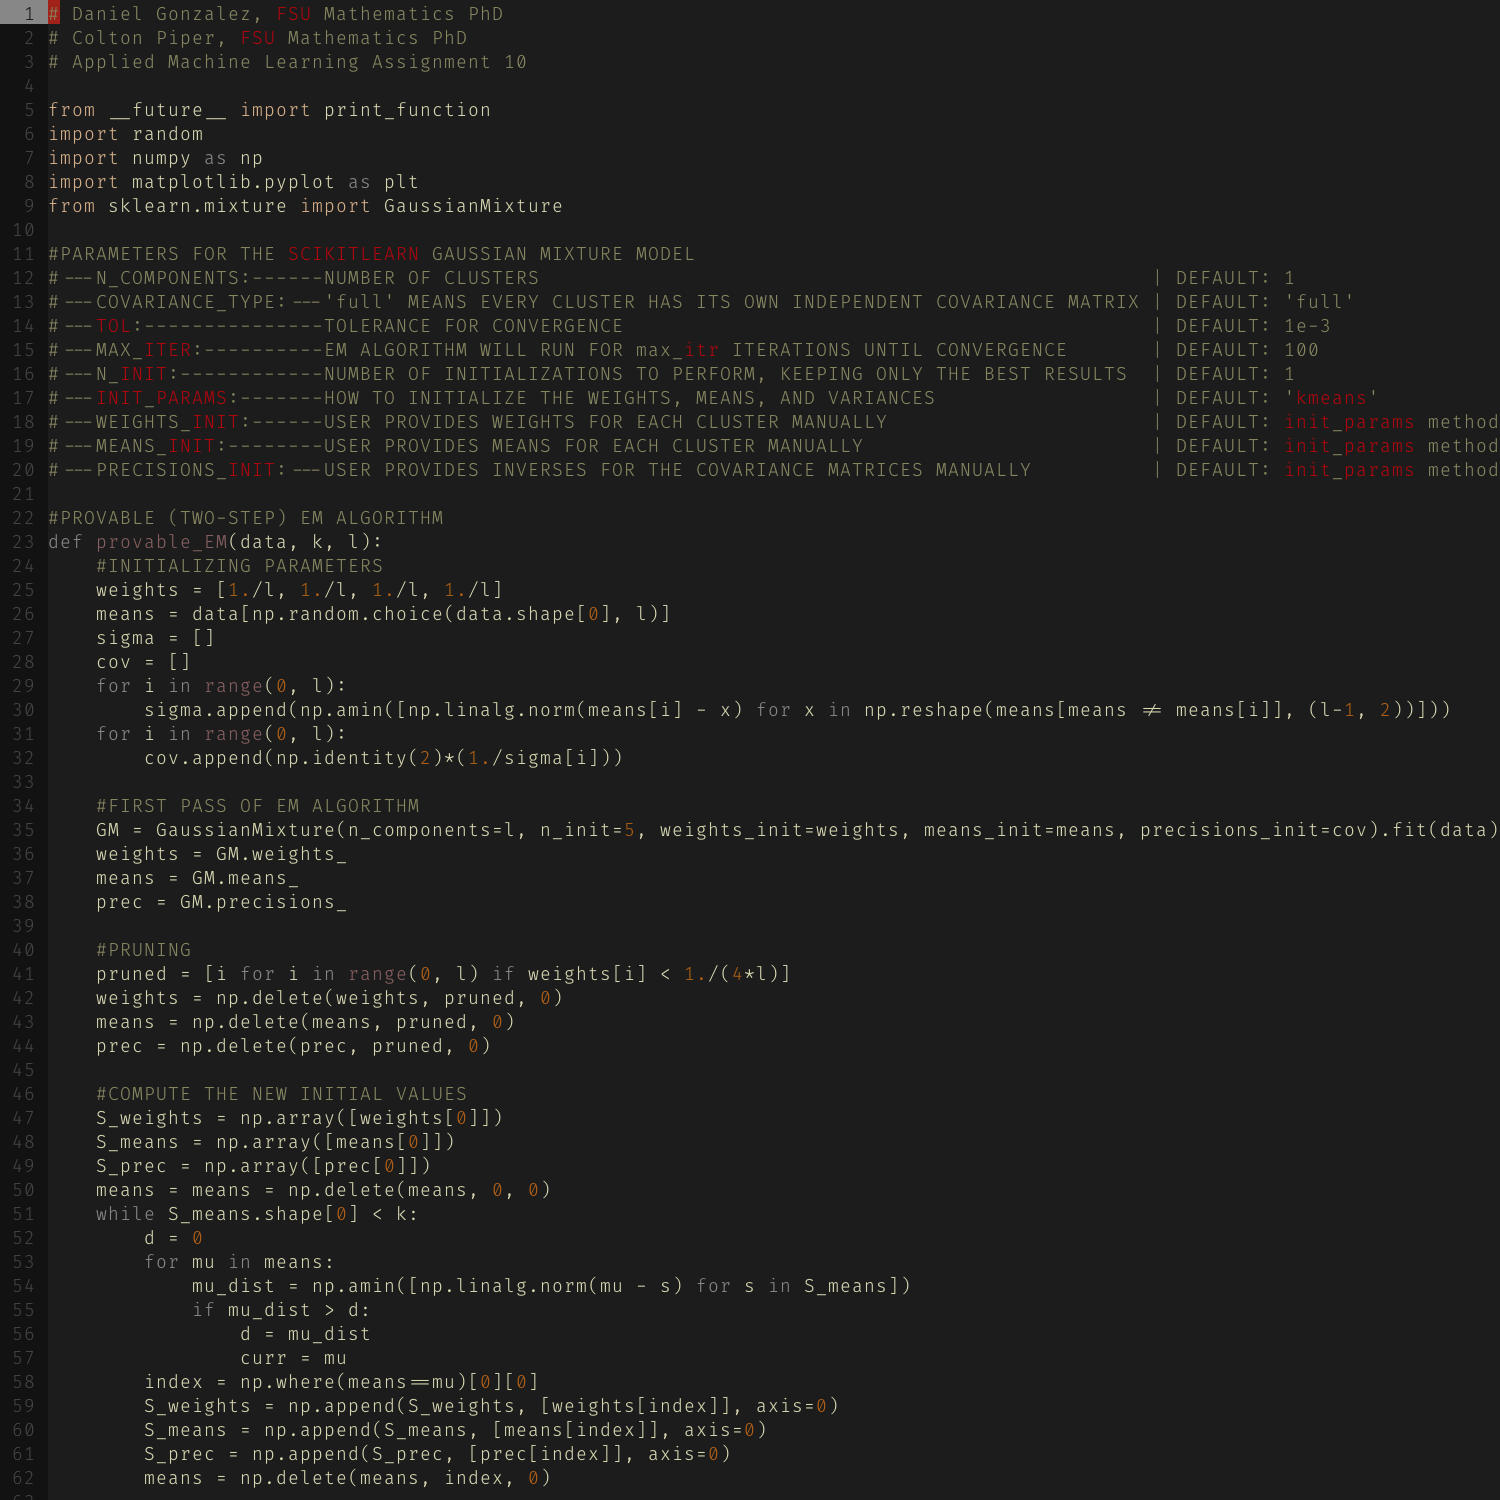
\includegraphics[scale=1.05]{./code/code1.png}
        \end{minipage}
    \end{figure}

\subsection{Mersenne Twister Code (\texttt{mersenne.hs})}
    \begin{figure}[H]
        \begin{minipage}{\textwidth}
            \centering
            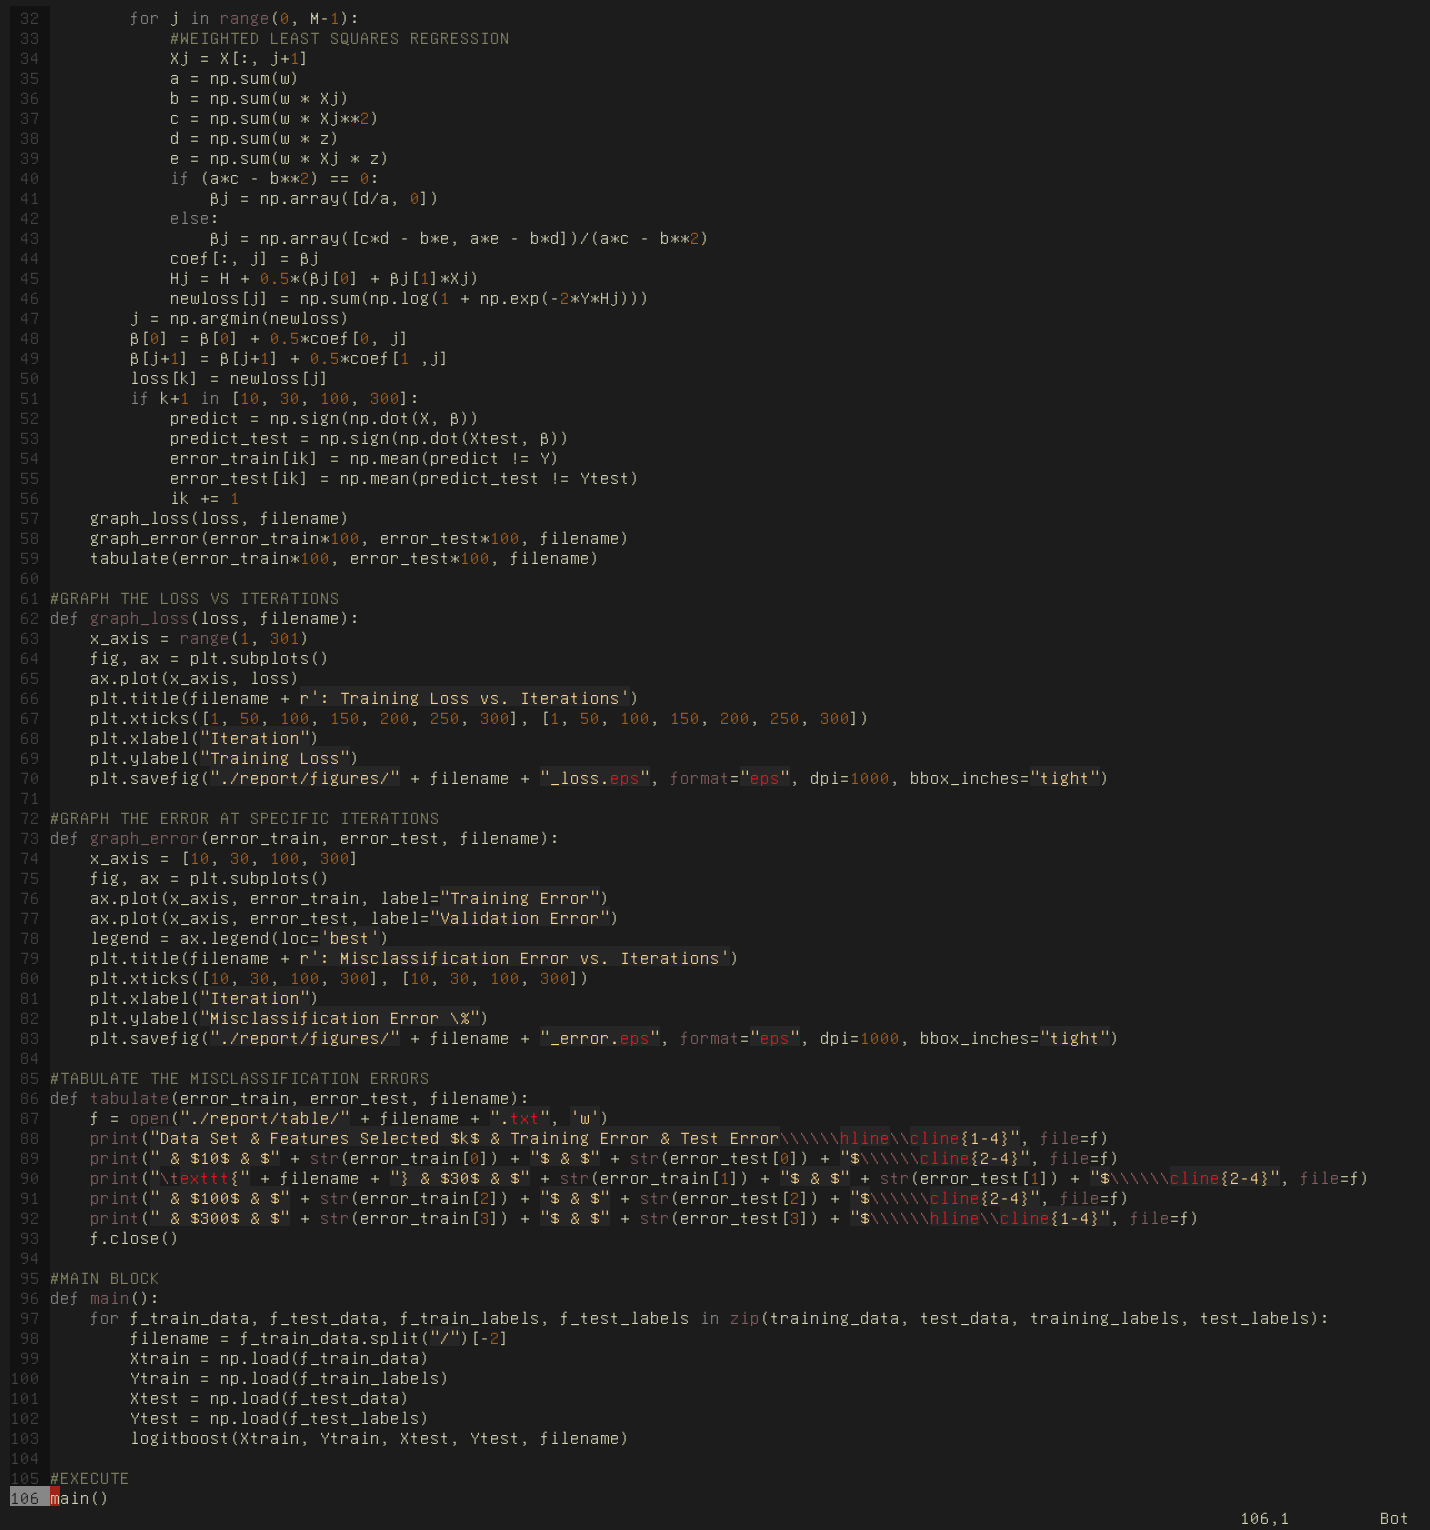
\includegraphics[scale=1]{./code/code2.png}
        \end{minipage}
    \end{figure}

\subsection{Halton Sequence Code (\texttt{halton.hs})}
    \begin{figure}[H]
        \begin{minipage}{\textwidth}
            \centering
            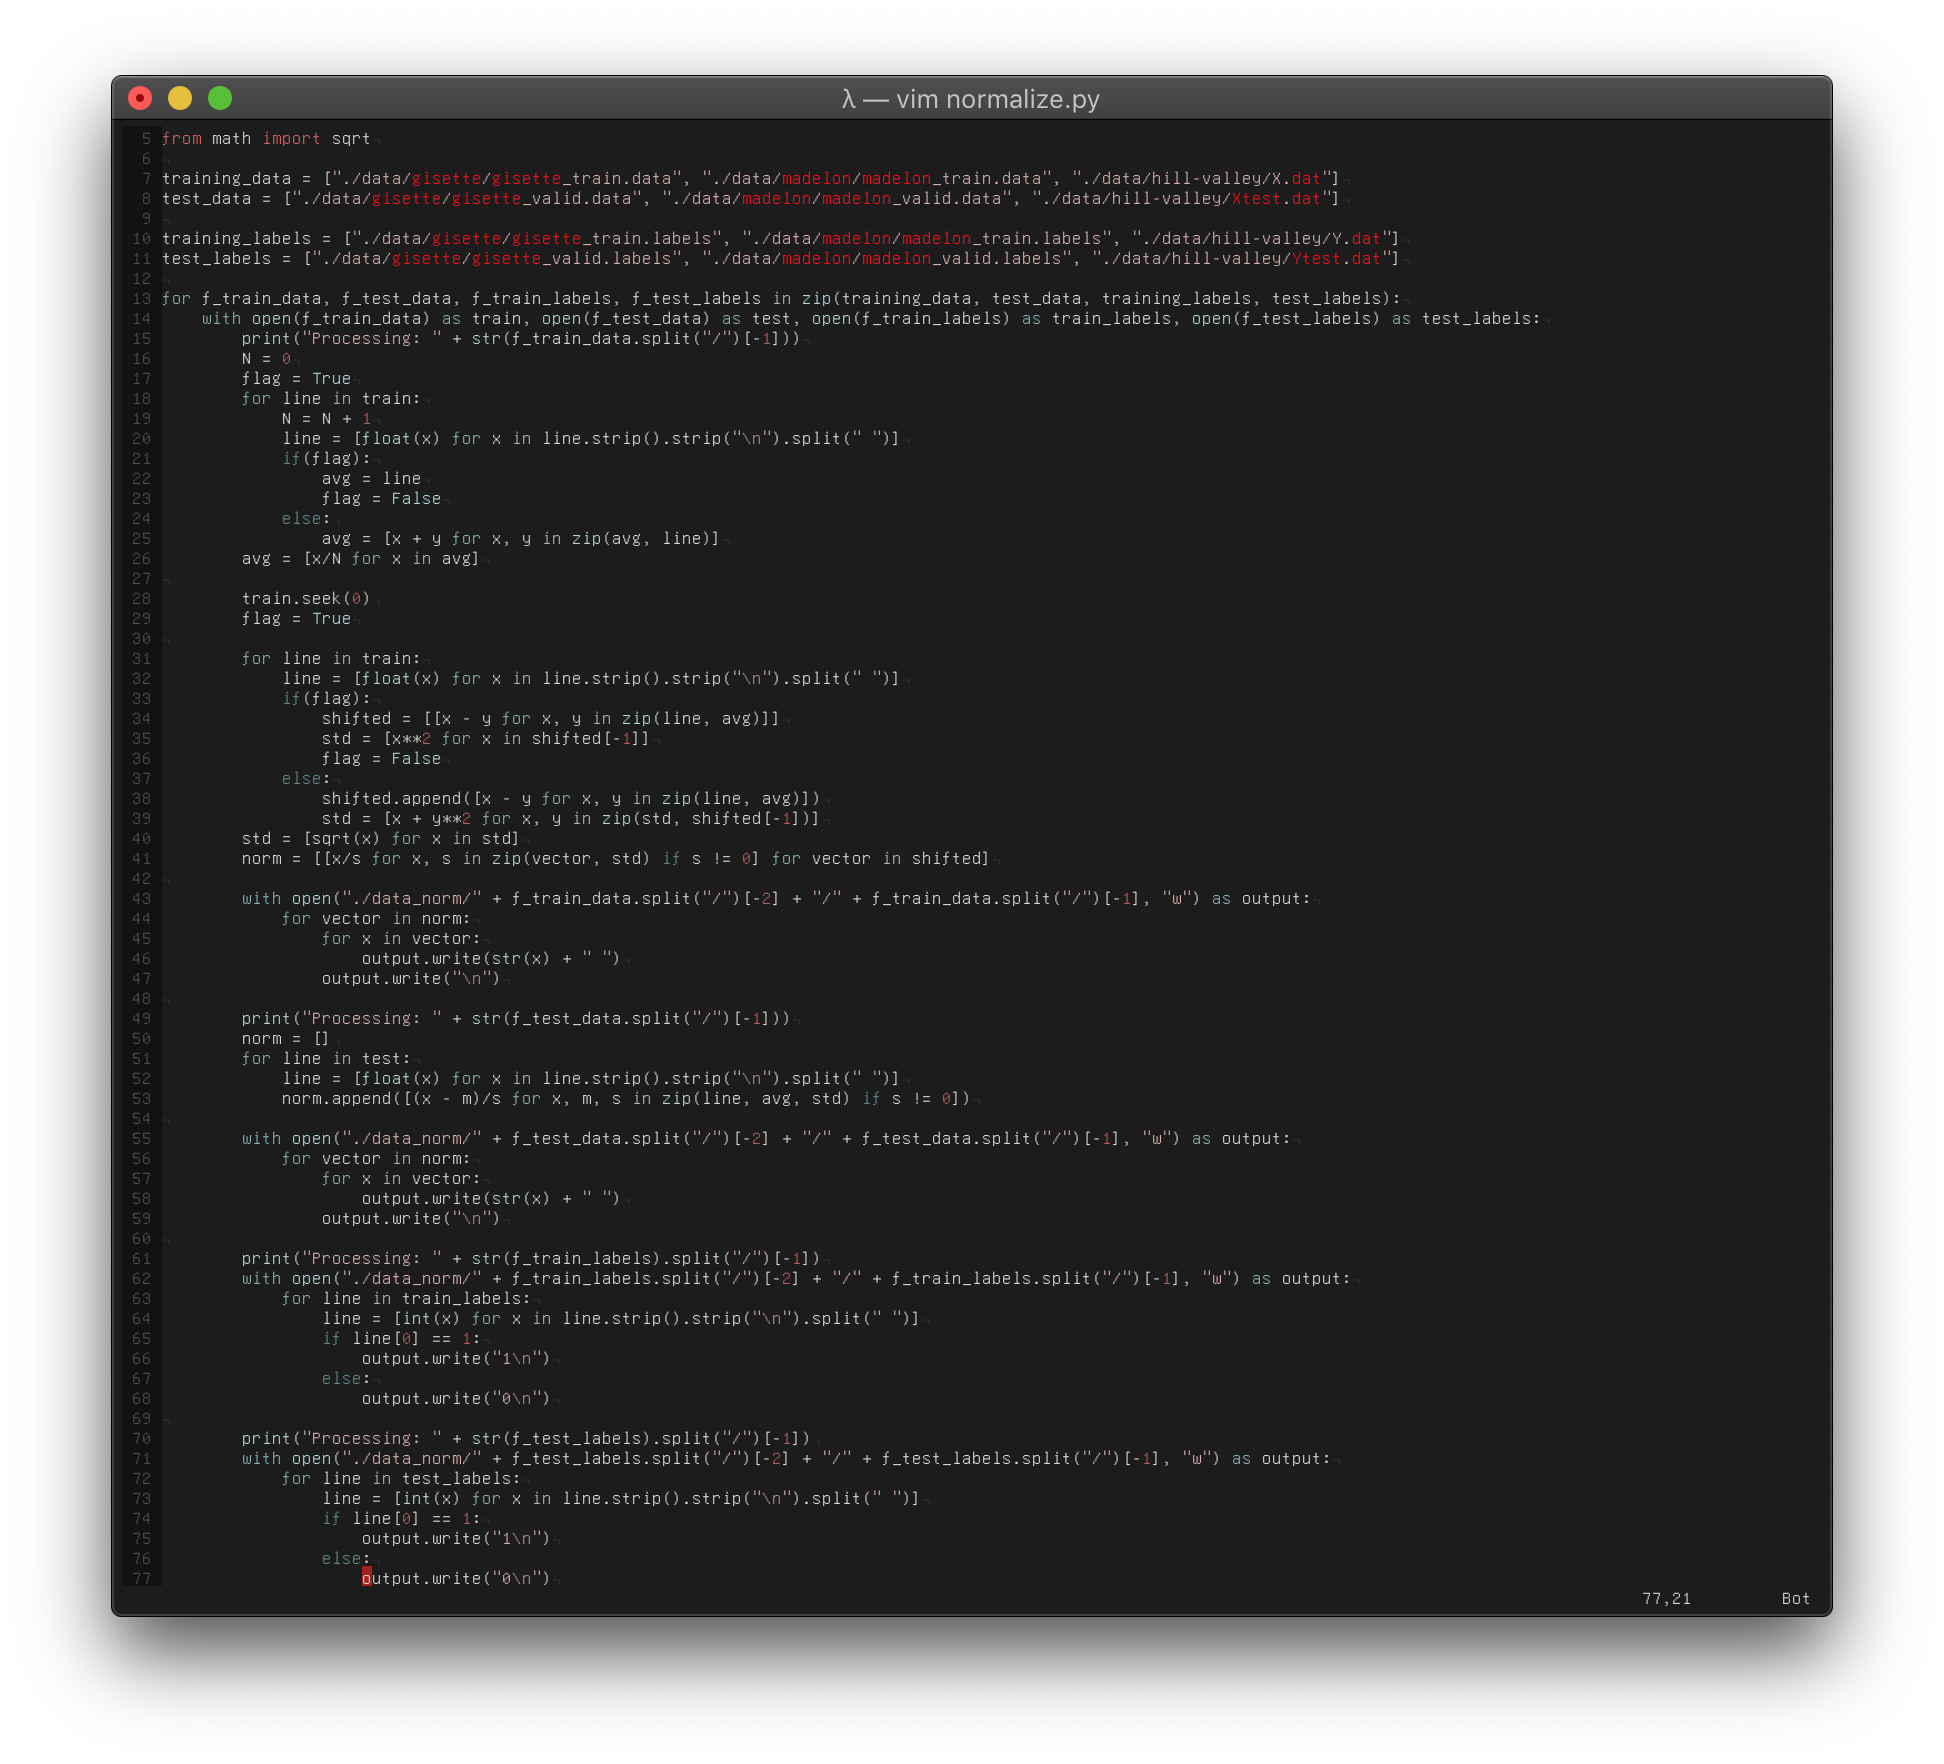
\includegraphics[scale=1.03]{./code/code3.png}
        \end{minipage}
    \end{figure}

\subsection{Monte Carlo Code (\texttt{MC.hs})}
    \begin{figure}[H]
        \begin{minipage}{\textwidth}
            \centering
            \includegraphics[scale=0.65]{./code/code4.png}
        \end{minipage}
    \end{figure}

\subsection{Random Quasi-Monte Carlo Code (\texttt{RQMC.hs})}
    \begin{figure}[H]
        \begin{minipage}{\textwidth}
            \centering
            \includegraphics[scale=0.83]{./code/code5.png}
        \end{minipage}
    \end{figure}

\subsection{2D Graphing (\texttt{graph.py})}
    \begin{figure}[H]
        \begin{minipage}{\textwidth}
            \centering
            \includegraphics[scale=0.55]{./code/code6.png}
        \end{minipage}
    \end{figure}

\subsection{3D Graphing (\texttt{graph.r})}
    \begin{figure}[H]
        \begin{minipage}{\textwidth}
            \centering
            \includegraphics[scale=0.95]{./code/code7.png}
        \end{minipage}
    \end{figure}

\end{document}
